\chapter{Introduction}
\label{chap1}

\section{Vibration problems in modern buildings}
Modern buildings have been showing increasing demand for faster construction, larger bay size and more flexible work space use in recent years. This demand usually leads to long spans, lightweight floor systems and reduced dividing partitions. The associated reduction of flexural stiffness, self weight attributed to unit floor area and structural damping of the floors has aroused a greater awareness of potential vibration problems when subjected to human activities.

A Building with vibration problems may cause an apprehension for the structural safety, loss of mental concentration and an unwell feeling among the people working inside \cite{bachmann2012vibration}. Such buildings are prone to be subject to more complaints than others. Unfortunately, once the construction is finished, it is very difficult to improve its dynamic performance by structural measures later on, as such modification is only possible by making major changes to the mass, stiffness or damping of the floor system. Therefore, it is significant to consider the human-induced vibration of floors at the conceptual stage.

\section{Rib-stiffened vaulted floor}
The rib-stiffened vaulted floor designed by BLOCK Research Group at ETH Zurich conforms to the trend of lightweight floor systems in modern buildings, it may be also confronted with accompanying vibration problems. A prototype of the vaulted floor element designed for the NEST HiLo project is shown in figure \ref{fig:prototype}. This unreinforced concrete floor consists of a thin funicular vault stiffened by a series of spandrel walls on its extrados. The structural prototype is completed with tension ties, which link the supports and absorb the horizontal thrusts of the funicular shell.
\begin{figure}[H]
\begin{subfigure}[b]{.9\textwidth}
  \centering
  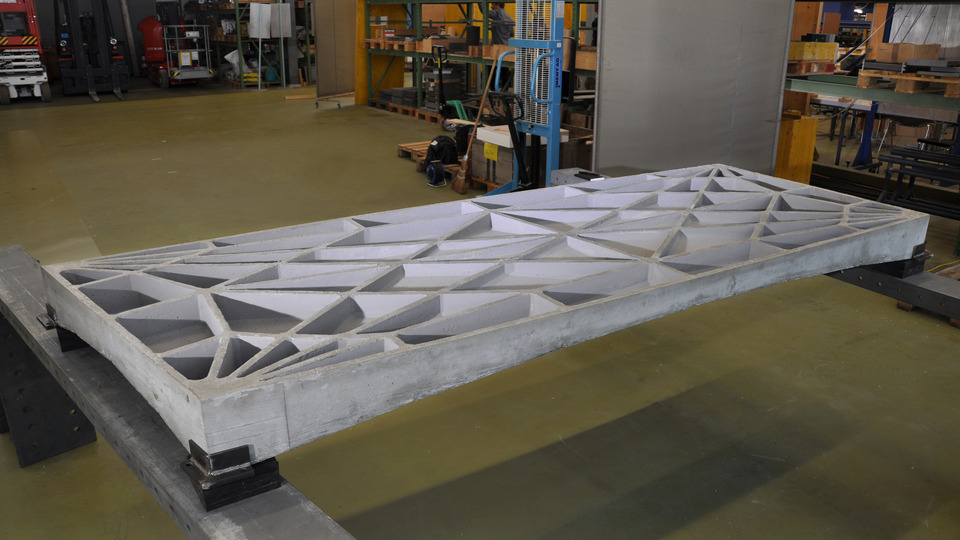
\includegraphics[width=.99\linewidth]{prototype1}
  \caption{The prototype before static experiment}
\end{subfigure}

\begin{subfigure}[b]{.9\textwidth}
  \centering
  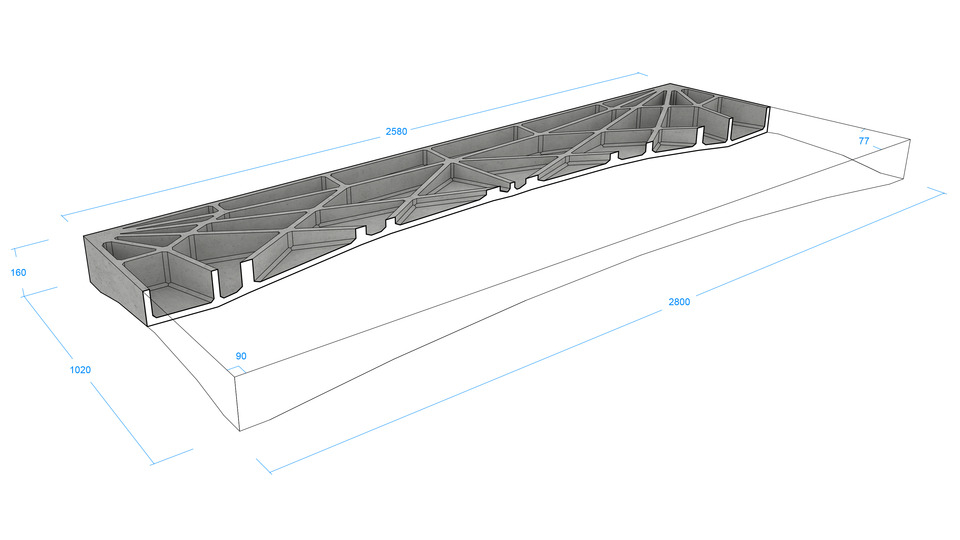
\includegraphics[width=.99\linewidth]{prototype2}
  \caption{Cross-section and dimensions}
\end{subfigure}

\caption{A prototype of the rib-stiffened valued floor \cite{prototype}}
\label{fig:prototype}
\end{figure}

The vaulted floor owns some unique geometric and modal features that differentiate itself from regular concrete and steel/concrete composite floors.
\begin{itemize}
    \item \textbf{Adequate stiffness achieved by ultra-lightweight construction}\\
    The geometry of the vault was found through the interactive form-finding process TNA (Thrust Network Analysis). Thanks to the inherent nature of TNA, the vault behaves as a compression-only shell under self-weight and dead load. The load transfer through compression is much more efficient than through bending. As a result, the floor would save more than 70\% of the weight compared to traditional, 25-30cm-thick concrete floor floors used in the construction of framed buildings and meanwhile keep deformations not higher than 1/500 of the span in the serviceability limit state \cite{lopez2014prototype}. 
    
    \item \textbf{High natural frequency}\\
    The high natural frequency is a direct consequence of the former feature. The natural frequency of a single degree of freedom system reads
    \begin{equation}
        f_n=\frac{1}{2\pi}\sqrt{\frac{k}{m}}
    \end{equation}
    It indicates that if the structure is so optimized that adequate stiffness remains while much mass is removed, the structure will show a high natural frequency. 
    
     The series of vaulted floors studied in this research (differ from this prototype in many aspects, but they share the same essential principles) have the fundamental natural frequencies ranging from 20 Hz to 100 Hz. The vaulted floor is a typical high frequency floor, in which resonant build up does not happen and the response is a series of rapidly decaying responses following each footfall. The cut-off frequency differentiating low frequency and high frequency floor is accepted by around 10 Hz \cite{smith2007design}\cite{willford2007predicting}. Then the vaulted floor would have been considered as very "dynamically stiff" when only judged from the aspect of the natural frequency.
    
    \item \textbf{Low modal mass}\\
    In the form-finding and optimization process of the vaulted floor much of its mass was removed from the middle, as it does not make much contribution to either stiffness or strength. On the contrary, a considerable amount of mass is distributed on the side due to the existence of stiffening ribs with high depth. Such muss distribution results in a very low modal mass. A solid rectangular floor has a modal mass of 25\% of the total mass (given that the mode shape is so normalized that the maximal item is 1) \cite{howard2007modal}, whereas only 1\%-7\% for a vaulted floor with constant thickness in both vault and ribs (see figure \ref{fig:geom-m12m}). 
    
    \item \textbf{Vault/ribs interaction}\\
    The ribs are intended to disperse the external load to vault and stiffen the vault locally in static cases. From the aspect of dynamics, the situation can be just the opposite. The vault has a more or less uniform mass distribution over the whole area, whereas the ribs have much higher mass and stiffness concentration near the edges. Therefore, the ribs are prone to vibrate locally in the middle with high amplitudes, the vault tends to stiffen the ribs in the middle and disperse the vibration to a larger region.
    
\end{itemize}

\section{Statement of problems}
Since the vaulted floor owns those unique features and their influences on its dynamic performance are not fully understood, or even not studied, there is an acute need for:
\begin{itemize}
    \item a fundamental understanding of the dynamic behavior of the vaulted floor
    \item improvement/optimization if the dynamic performance turns out to be unsatisfactory
\end{itemize}

\section{Objectives}
This study is limited to explore the dynamic performance of the vaulted floor under one person walking excitation. In pursuit of a fundamental understanding of its dynamic behavior, the following objectives must be firstly addressed in the study:
\begin{itemize}
    \item to develop an analysis procedure for dynamic response, allowing fast, accurate and robust solution of dynamic process;
    \item to implement suitable approaches for evaluation of vibration perception;
    \item to identify key parameters that influence the dynamic performance by parametric study and sensitivity analysis, more importantly, to understand how they influence and why they influence the performance in that way; and,
    \item to find qualitative and quantitative relations among geometry, modal property and dynamic performance. 
\end{itemize}

Based on the understanding obtained above, improvement/optimization can be achieved if the following objectives are realized:
\begin{itemize}
    \item to find the "best" mass and stiffness distribution under certain constraints (e.g. constant mass, allowable thickness ratio, etc.) either through oriented trial and error or automatic optimization; and,
    \item to consider and demonstrate the feasibility of attaining such mass and stiffness distribution in reality.
\end{itemize}


\section{Thesis structure}
This master's thesis is composed of 6 chapters.

Chapter 1 introduces the importance of the study on dynamic performance of floors in modern buildings and provides background information about the rib-stiffened vaulted floor. The statement of problems and objectives are defined.

Chapter 2 reviews the evaluation methods for the dynamic performance of floors and the state of the art in design codes and research.

Chapter 3 elaborates the methodology for the evaluation of dynamic performance. Basic modeling assumptions are clarified and analysis procedure for the dynamic response is introduced.

Chapter 4 delivers the results of dynamic analysis. The calibration of the results from modal superposition and from Abaqus is conducted. The rest of this chapter reveals the relations among geometric parameters, modal properties and dynamic performance. 

Chapter 5 presents two possible ways to improve the dynamic performance. One is based on the acquired understanding of the floor's dynamic behavior from previous analysis, the other is a surrogate model based automated optimization.

Chapter 6 concludes the main findings in this thesis with an outlook on further research possibilities. 



























